%%%%%%%%%%%%%%%%%%%%%%%%%%%%%%%%%%%%%%%%%
% Beamer Presentation
% LaTeX Template
% Version 1.0 (10/11/12)
%
% This template has been downloaded from:
% http://www.LaTeXTemplates.com
%
% License:
% CC BY-NC-SA 3.0 (http://creativecommons.org/licenses/by-nc-sa/3.0/)
%
%%%%%%%%%%%%%%%%%%%%%%%%%%%%%%%%%%%%%%%%%

%----------------------------------------------------------------------------------------
%	PACKAGES AND THEMES
%----------------------------------------------------------------------------------------

\documentclass{beamer}
\usefonttheme[onlymath]{serif}

\mode<presentation> {

% The Beamer class comes with a number of default slide themes
% which change the colors and layouts of slides. Below this is a list
% of all the themes, uncomment each in turn to see what they look like.

%\usetheme{default}
%\usetheme{AnnArbor}
%\usetheme{Antibes}
%\usetheme{Bergen}
%\usetheme{Berkeley}
%\usetheme{Berlin}
%\usetheme{Boadilla}
%\usetheme{CambridgeUS}
%\usetheme{Copenhagen}
%\usetheme{Darmstadt}
%\usetheme{Dresden}
%\usetheme{Frankfurt}
%\usetheme{Goettingen}
%\usetheme{Hannover}
%\usetheme{Ilmenau}
%\usetheme{JuanLesPins}
%\usetheme{Luebeck}
\usetheme{Madrid}
%\usetheme{Malmoe}
%\usetheme{Marburg}
%\usetheme{Montpellier}
%\usetheme{PaloAlto}
%\usetheme{Pittsburgh}
%\usetheme{Rochester}
%\usetheme{Singapore}
%\usetheme{Szeged}
%\usetheme{Warsaw}

% As well as themes, the Beamer class has a number of color themes
% for any slide theme. Uncomment each of these in turn to see how it
% changes the colors of your current slide theme.

%\usecolortheme{albatross}
%\usecolortheme{beaver}
%\usecolortheme{beetle}
%\usecolortheme{crane}
%\usecolortheme{dolphin}
%\usecolortheme{dove}
%\usecolortheme{fly}
%\usecolortheme{lily}
%\usecolortheme{orchid}
%\usecolortheme{rose}
%\usecolortheme{seagull}
%\usecolortheme{seahorse}
%\usecolortheme{whale}
%\usecolortheme{wolverine}

%\setbeamertemplate{footline} % To remove the footer line in all slides uncomment this line
%\setbeamertemplate{footline}[page number] % To replace the footer line in all slides with a simple slide count uncomment this line

%\setbeamertemplate{navigation symbols}{} % To remove the navigation symbols from the bottom of all slides uncomment this line
}

\usepackage{graphicx} % Allows including images
\usepackage{booktabs} % Allows the use of \toprule, \midrule and \bottomrule in tables

\usepackage{multirow}
\usepackage{xcolor}
\usepackage{colortbl}
\usepackage{xspace}
\usepackage{bbm}
\usepackage{amsfonts}

\newcolumntype{g}{>{\columncolor{black!5}}c}
\newcolumntype{f}{>{\columncolor{black!5}}r}
\newcolumntype{L}[1]{>{\columncolor{black!5}}m{#1}}
\usepackage{tikz}
\usetikzlibrary{shapes}
\usetikzlibrary{arrows}
\usetikzlibrary{positioning}


\title[Content in DL Sum.]{Content Selection in Deep Learning Models of Summarization} % The short title appears at the bottom of every slide, the full title is only on the title page

\author[Chris Kedzie]{\textbf{Chris Kedzie}, Kathy McKeown, and Hal Daum\'e III (UMD/MSR)} % Your name
\institute[Columbia U.] % Your institution as it will appear on the bottom of every slide, may be shorthand to save space
{
Columbia University \\ % Your institution for the title page
\medskip
\textit{kedzie@cs.columbia.edu} % Your email address
}
\date{\today} % Date, can be changed to a custom date

\begin{document}

\begin{frame}
\titlepage 
\end{frame}

%\begin{frame}{Generic Single Document Summarization}
%
%  \textbf{Generic Single Document Summarization}
%
%  \begin{itemize}
%    \item Most research has focused on news.
%    \item Recent increased interest since 2016. \textbf{Why?}
%      \begin{itemize}
%        \item CNN/DailyMail Dataset (300k document summary pairs)
%        \item More recently the Newsroom dataset offers 1.3 million training 
%              examples
%        \item General purpose sequence-to-sequence transduction models from the
%              Neural Machine Translation community
%      \end{itemize}
%    \item <2-> Will this approach work?
%      \begin{itemize}
%        \item<2-> With enough data, we can treat the model as a black box.
%        \item<2-> Avoid having to specify summarization model task which is 
%                  complex/unknown/underspecified.
%      \end{itemize}
%    \item<3-> \textbf{This Talk:} Reasons to be skeptical that this will work.
%  \end{itemize}      
%\end{frame}
%
%
%\begin{frame}{How do deep learning models learn what's important?}
%    
%    \begin{itemize}
%        \item What sentence representations are best for content selection?
%                \uncover<2->{\alert<2->{ Simpler is better.}}
%        \item What sentence selection architectures are best for content selection?
%                \uncover<2->{\alert<2->{ Simpler is better.}}
%        \item What are the most significant learning signals in the data?\\
%                \uncover<3->{\alert<3->{Word-level semantics only modestly useful. Structural/positional signals are more important. }}
%    \end{itemize}
%
%\end{frame}

\begin{frame}{Deep learning for Extractive Summarization}

  \begin{itemize}
    \item[--] Lots of recent research activity using deep learning for 
              summarization!  \\
              ~\\
              ~\\
              ~\\
    \item[--] Unclear what model design choices are most effective.\\
              \uncover<2>{\alert<2>{We perform a comparison of recent 
              architectures and propose our own simplificiations.\\}}
              ~\\
    \item[--] Unclear what are the most important signals in the data for 
              learning.\\
              \uncover<2>{\alert<2>{We perform a several experimental probes
              to understand the contributions of lexical semantics vs.
              structure/discourse.}}
  \end{itemize}
  
\end{frame}


\begin{frame}{Talk Outline}
  \tableofcontents
\end{frame}

\section{Problem Definition}

\begin{frame}{Extractive Summarization as Sequence Tagging}
  \begin{center}
    \begin{tikzpicture}
      \node<1-2>[inner sep=0pt] (bg) at (0,0)
        {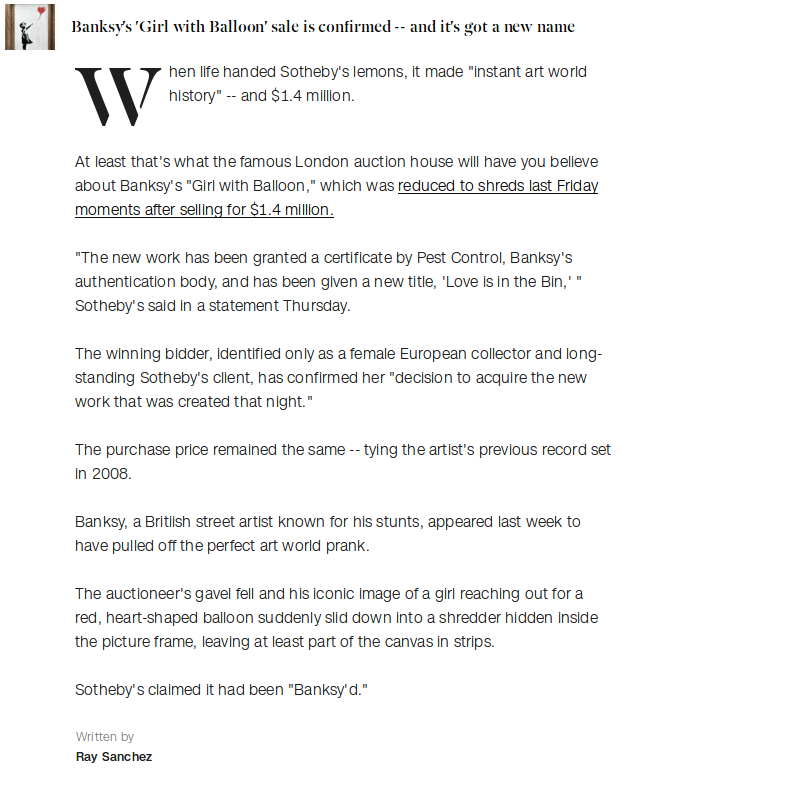
\includegraphics[width=.65\textwidth]{2_problem_definition/images/article_before.png}};
      \node<3>[inner sep=0pt] (bg) at (0,0)
        {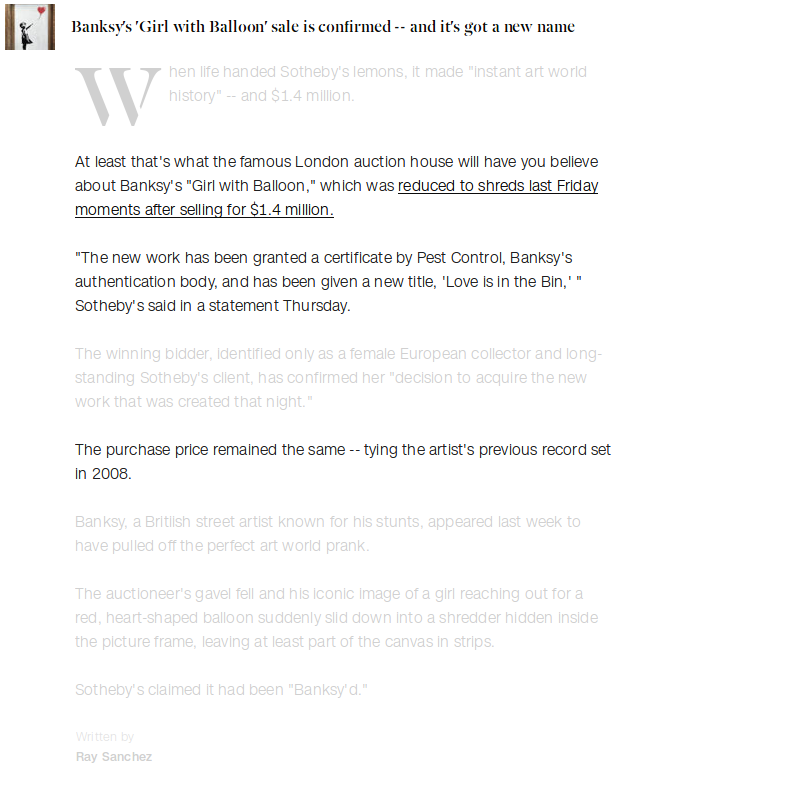
\includegraphics[width=.65\textwidth]{2_problem_definition/images/article_after.png}};
      \node (s1) at (4,2.8) 
           {\huge $s_1 \;\uncover<2->{\rightarrow y_1}\uncover<3->{=0}$};
      \node (s2) at (4, 2.0) 
           {\huge $s_2 \;\uncover<2->{\rightarrow y_2}\uncover<3->{=1}$};
      \node (s3) at (4, 1.2)
           {\huge $s_3 \;\uncover<2->{\rightarrow y_3}\uncover<3->{=1}$};
      \node (s4) at (4, 0.4)
           {\huge $s_4 \;\uncover<2->{\rightarrow y_4}\uncover<3->{=0}$};
      \node (s5) at (4,-0.4)
           {\huge $s_5 \;\uncover<2->{\rightarrow y_5}\uncover<3->{=1}$};
      \node (s6) at (4,-1.2)
           {\huge $s_6 \;\uncover<2->{\rightarrow y_6}\uncover<3->{=0}$};
      \node (s7) at (4,-2.0)
           {\huge $s_7 \;\uncover<2->{\rightarrow y_7}\uncover<3->{=0}$};
      \node (s8) at (4,-2.8)
           {\huge $s_8 \;\uncover<2->{\rightarrow y_8}\uncover<3->{=0}$};
    \end{tikzpicture}
  \end{center}
\end{frame}




\AtBeginSection[]{
    \begin{frame}<beamer>
        \frametitle{Talk Outline}
        \tableofcontents[currentsection]
    \end{frame}
}
\section{Architecture}

\begin{frame}{Summarizer Architecture}
  \begin{center}
    \begin{tikzpicture}
      \node at (0.4,-.75) {Sentence 1};
      \node at (4.9,-.75) {Sentence 2};
      \node at (8.9,-.75) {Sentence 3};
      \node (w1) at (0,0) 
      {\large $\uncover<2->{\textsc{Enc}\left(}w^{(1)}_1,
         w^{(1)}_2, w^{(1)}_3\uncover<2->{\right)}$};

      \node (w2) at (4.5,0) 
      {\large $\uncover<2->{\textsc{Enc}\left(}w^{(2)}_1, 
         w^{(2)}_2, w^{(2)}_3\uncover<2->{ \right)}$};
      \node (w3) at (8.6,0) 
      {\large $\uncover<2->{\textsc{Enc}\left(}w^{(3)}_1, 
         w^{(3)}_2\uncover<2->{\right)}$};

      \node (s1) at (3,2) {\large $\uncover<3->{s_1}$};
      \node (s2) at (4,2) {\large $\uncover<3->{s_2}$};
      \node (s3) at (5,2) {\large $\uncover<3->{s_3}$};
      \uncover<3->{  
        \draw[->,thick] (w1.north) -- (s1.south); 
        \draw[->,thick] (w2.north) -- (s2.south);
        \draw[->,thick] (w3.north) -- (s3.south);
      }

      \uncover<4->{
        \node (ext) at (3.6,2) {\large $\textsc{Ext}\Big( 
        \quad\quad\quad\;\;\;\;\;\;\;\;\;\;\; \Big)$};
      }
      \uncover<5->{
        \node (y1) at (3,3.5) {\large $y_1$};
        \node (y2) at (4,3.5) {\large $y_2$};
        \node (y3) at (5,3.5) {\large $y_3$};
        \draw[->,thick] (s1.north) -- (y1.south);
        \draw[->,thick] (s2.north) -- (y2.south);
        \draw[->,thick] (s3.north) -- (y3.south);
      }

    \end{tikzpicture}
  \end{center}
\end{frame}


\begin{frame}{Sentence Encoders}
 \begin{columns}[t]
  \column{.32\textwidth}
   \centering
   Averaging Encoder\\~\\
   \includegraphics[]{images/avg_encoder.pdf}\\
  \column{.32\textwidth}
   \centering
   RNN Encoder\\~\\
   \includegraphics[]{images/rnn_encoder.pdf}\\
  \column{.32\textwidth}
   \centering
   CNN Encoder\\~\\
   \includegraphics[]{images/cnn_encoder.pdf}\\
 \end{columns}

~\\
We use pretrained (Wikipedia/Gigaword) Glove word embeddings.

\end{frame}
%
%\begin{frame}{Sentence Extractor}
%  \textbf{Previous Work}\\~\\
%  ~~ -- \textbf{Cheng and Lapata Extractor} ~~ seq2seq inspired architecture 
%                                               (Cheng and Lapata, 2016)\\
%  ~~ -- \textbf{SummaRunner Extractor} ~~ RNN inspired architecture with 
%                                          document and summary representations 
%                                          (Nallapati et al., 2016)\\
%  ~\\~\\
%  \textbf{Our Extractors}\\~\\
%  ~~ -- \alert<2>{\textbf{RNN Extractor}} ~~ Simplified version of SummaRunner \\
%  ~~ -- \textbf{Seq2Seq Extractor} ~~ seq2seq (with attention) inspired 
%                                      architecture \\
%\end{frame}


\begin{frame}{Sentence Extractors}
 \begin{columns}[t]
  \column{.4\textwidth}
  \only<1,2,4>{
   \centering
   SummaRunner Extractor\\
   (Nallapati et al. 2016)\\
   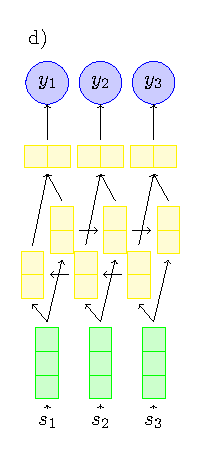
\includegraphics[scale=.65]{images/sr_extractor.pdf}\\
   RNN Extractor (ours)\\
   \includegraphics[scale=.65]{images/rnn_extractor.pdf}
}
\only<3>{
    Cheng \& Lapata Model
    \begin{enumerate}
        \item Offset encoder/decoder inputs, no attention
        \item Complex interaction between previous extraction prediction and 
            decoder input.
    \end{enumerate}
    ~\\~\\
    Seq2Seq Model
    \begin{enumerate}
        \item Simple dot-product attention
        \item \textbf{(Conditionally) independent} extraction decisions
    \end{enumerate}
}
  \column{.6\textwidth}
  \only<1,3,4>{
   \centering
   Cheng \& Lapata Extractor\\
   (Cheng and Lapata, 2016)\\
   \includegraphics[scale=.65]{images/cl_extractor.pdf}\\
   Seq2Seq Extractor (ours)\\
   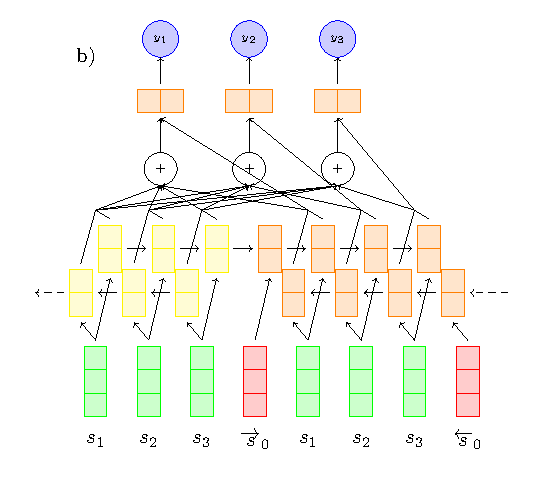
\includegraphics[scale=.65]{images/s2s_extractor.pdf}
   }
   \only<2>{
        SummaRunner Model
        \begin{itemize}
        \item Internal representations of document similarity and summary novelty
        \item Explicit representation of position
        \item Complex dependencies between extraction decisions
        \end{itemize}
~\\
~\\
        RNN Model
        \begin{itemize}
            \item \sout{Internal representations of document similarity and summary novelty}
            \item \sout{Explicit representation of position}
            \item \textbf{(Conditionally) independent} extraction decisions
        \end{itemize}

   }
 \end{columns}

\end{frame}


%\begin{frame}{Sentence Encoder}
%  \textbf{Averaging Encoder} ~~ $s = $ average of word embeddings \\
%  ~\\
%  \textbf{RNN Encoder} ~~ $s = $ final states of bi-directional GRU.\\
%  ~\\
%  \textbf{CNN Encoder} ~~ $s = $ 1-d convolutions over word embeddings.\\
%  ~\\~\\
%  * Word embeddings are fixed Glove embeddings (trained on Wikipedia and 
%    Gigaword). 
%\end{frame}
%

%
%\begin{frame}{RNN Extractor}
%  \begin{columns}
%    \begin{column}{0.5\textwidth}
%      \documentclass[crop,tikz]{standalone}
\usetikzlibrary{shapes}
\usetikzlibrary{arrows}
\usetikzlibrary{positioning}

\begin{document}
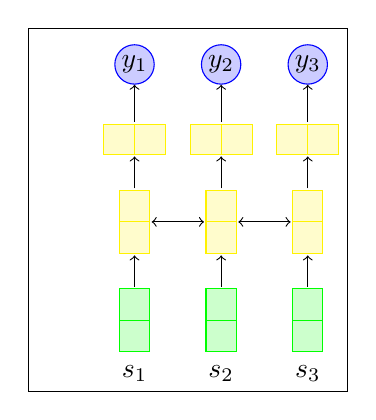
\begin{tikzpicture}[
  hid/.style 2 args={
    rectangle split,
    draw=#2,
    rectangle split parts=#1,
    fill=#2!20,
    outer sep=.25mm},
  mlp/.style 2 args={
    rectangle split,
    rectangle split horizontal,
    draw=#2,
    rectangle split parts=#1,
    fill=#2!20,
    outer sep=.25mm}
]

 % Comment out this line to remove border.
 \draw[draw=black] (-.25, 4.21) rectangle (3.8, -.4);

 \foreach \step in {1,...,3} {
   \node (i\step) at (1.1*\step, -.18) {$s_\step$};
   \node[hid={2}{green}] (e\step) at (1.1*\step, .5) {};    
 }
  
 \foreach \step in {1,...,3} {
   \node[hid={2}{yellow}] (h\step) at (1.1 *\step, 1.75) {};    
   \draw[->] (e\step.north) -> (h\step.south);
   
   \node[mlp={2}{yellow}] (g\step) at (1.1 *\step, 2.8) {};    
   \node[circle, draw=blue, fill=blue!20,minimum size=5mm] (y\step) 
       at (1.1 *\step, 3.75) {};
   \node at (1.1 *\step, 3.75) {$y_\step$};    
   \draw[->] (g\step.north) -> (y\step.south);
   \draw[->] (h\step.north) -> (g\step.south);
 }

 \foreach \last/\next in {1/2, 2/3} {
   \draw[<->] (h\last.east) -> (h\next.west);
 }


\end{tikzpicture}
\end{document}

%    \end{column}
%    \begin{column}{0.5\textwidth}
%      \uncover<2->{
%            $p(y|h) = \prod_{i=1}^n p(y_i|h)$ 
%      }
%    \end{column}
%  \end{columns}
%\end{frame}
%
%\begin{frame}{Sentence Extractor}
%  \textbf{Previous Work}\\~\\
%  ~~ -- \textbf{Cheng and Lapata Extractor} ~~ seq2seq inspired architecture 
%                                               (Cheng and Lapata, 2016)\\
%  ~~ -- \textbf{SummaRunner Extractor} ~~ RNN inspired architecture with 
%                                          document and summary representations 
%                                          (Nallapati et al., 2016)\\
%  ~\\~\\
%  \textbf{Our Extractors}\\~\\
%  ~~ -- \textbf{RNN Extractor} ~~ Simplified version of SummaRunner \\
%  ~~ -- \alert{\textbf{Seq2Seq Extractor}} ~~ seq2seq (with attention) inspired
%                                              architecture \\
%\end{frame}
%
%
%
%\begin{frame}{Seq2Seq Extractor}
%    \begin{columns}
%        \begin{column}{0.5\textwidth}
%            \documentclass[tikz,border=10pt]{standalone}
\usetikzlibrary{shapes}
\usetikzlibrary{arrows}
\usetikzlibrary{positioning}
\begin{document} 

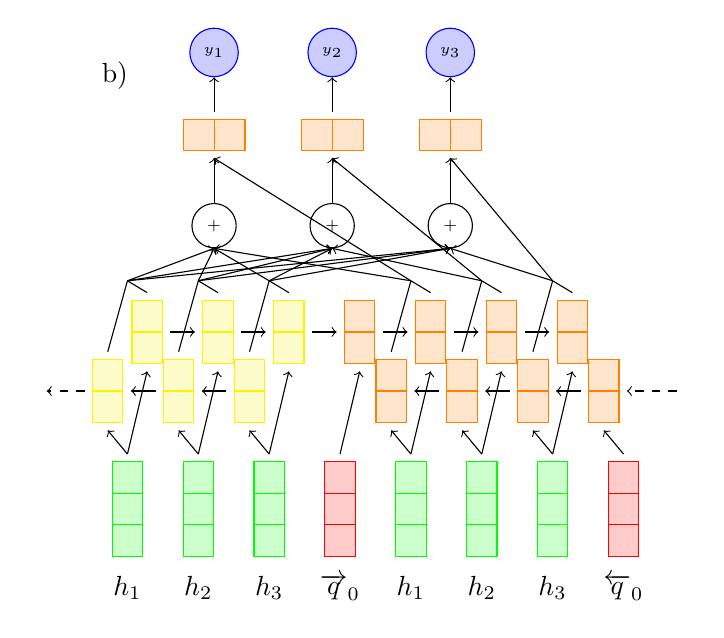
\begin{tikzpicture}[
  hid/.style 2 args={
    rectangle split,
    draw=#2,
    rectangle split parts=#1,
    fill=#2!20,
    outer sep=1mm},
  mlp/.style 2 args={
    rectangle split,
    rectangle split horizontal,
    draw=#2,
    rectangle split parts=#1,
    fill=#2!20,
    outer sep=1mm}
]

  \node [anchor=west] (label) at (.45, 4.5) {b)};

  \foreach \i [count=\step from 1] in {$h_1$, $h_2$, $h_3$} {
    \node (i\step) at (.9*\step, -2) {\i};
    \node[hid={3}{green}] (e\step) at (.9*\step, -1) {};    
  }
  \node (i4) at (.9*4, -2) {$\overrightarrow{q}_0$};
  \node[hid={3}{red}] (e4) at (.9*4, -1) {};    
  \foreach \i [count=\step from 5] in {$h_1$, $h_2$, $h_3$} {
    \node (i\step) at (.9*\step, -2) {\i};
    \node[hid={3}{green}] (e\step) at (.9*\step, -1) {};    
  }
  \node (i8) at (.9*8, -2) {$\overleftarrow{q}_0$};
  \node[hid={3}{red}] (e8) at (.9*8, -1) {};    

  \foreach \step in {1,...,3} {
    \node[hid={2}{yellow}] (h_r_\step) at (-.25 + .9 *\step, .5) {};    
    \node[hid={2}{yellow}] (h_f_\step) at (.25 + .9 *\step, 1.25) {};    
    \draw[->] (e\step.north) -> (h_f_\step.south);
    \draw[->] (e\step.north) -> (h_r_\step.south);
%    \node[mlp={2}{yellow}] (h_\step) at (.9 *\step, 2.5) {};    
%    \node[circle, draw=blue, fill=blue!20] (y_\step) at (.9 *\step, 3.75) {$y_\step$};    
%    \draw[->] (h_\step.north) -> (y_\step.south);
%    \draw[->] (h_f_\step.north) -> (h_\step.south);
%    \draw[->] (h_r_\step.north) -> (h_\step.south);
  }

  \foreach \step in {5,...,8} {
    \node[hid={2}{orange}] (h_r_\step) at (-.25 + .9 *\step, .5) {};    
    \draw[->] (e\step.north) -> (h_r_\step.south);
  }
  \foreach \step in {4,...,7} {
    \node[hid={2}{orange}] (h_f_\step) at (.25 + .9 *\step, 1.25) {};    
    \draw[->] (e\step.north) -> (h_f_\step.south);
%    \draw[->] (e\step.north) -> (h_r_\step.south);
%    \node[mlp={2}{yellow}] (h_\step) at (.9 *\step, 2.5) {};    
%    \node[circle, draw=blue, fill=blue!20] (y_\step) at (.9 *\step, 3.75) {$y_\step$};    
%    \draw[->] (h_\step.north) -> (y_\step.south);
%    \draw[->] (h_f_\step.north) -> (h_\step.south);
%    \draw[->] (h_r_\step.north) -> (h_\step.south);

  }

  \draw[->] (h_f_1.east) -> (h_f_2.west);
  \draw[->] (h_f_2.east) -> (h_f_3.west);
  \draw[->] (h_f_3.east) -> (h_f_4.west);
  \draw[->] (h_f_4.east) -> (h_f_5.west);
  \draw[->] (h_f_5.east) -> (h_f_6.west);
  \draw[->] (h_f_6.east) -> (h_f_7.west);
 
  \draw[->] (h_r_3.west) -> (h_r_2.east);
  \draw[->] (h_r_2.west) -> (h_r_1.east);
  \node (lborder) at (-.25 + .9 * 0, .5) {};
  \node (rborder) at (-.1 + .9 * 9, .5) {};
  \draw[->,dashed] (h_r_1.west) -- (lborder);
  \draw[->,dashed] (rborder) -- (h_r_8.east);
  \draw[->] (h_r_8.west) -> (h_r_7.east);
  \draw[->] (h_r_7.west) -> (h_r_6.east);
  \draw[->] (h_r_6.west) -> (h_r_5.east);

  \node[circle,draw=black] (attn1) at (2, 2.6) {\tiny$+$};    
  \node[circle,draw=black] (attn2) at (3.5, 2.6) {\tiny$+$};    
  \node[circle,draw=black] (attn3) at (5, 2.6) {\tiny$+$};    
  
  \node[mlp={2}{orange}] (h1) at (2, 3.75) {};
  \node[mlp={2}{orange}] (h2) at (3.5, 3.75) {};
  \node[mlp={2}{orange}] (h3) at (5, 3.75) {};
  \node[circle, draw=blue, fill=blue!20] (y1) at (2, 4.8) {\tiny $y_1$};    
  \node[circle, draw=blue, fill=blue!20] (y2) at (3.5, 4.8) {\tiny $y_2$};    
  \node[circle, draw=blue, fill=blue!20] (y3) at (5, 4.8) {\tiny $y_3$};    

  \foreach \step in {1,...,3} {
      \node (m\step) at (\step * .9, 1.9) {};
      \path[draw=black,-] (h_f_\step.north) -- (m\step.center);
      \path[draw=black,-] (h_r_\step.north) -- (m\step.center);
      \foreach \stepj in {1,...,3} {
          \path[draw=black,->] (m\step.center) -- (attn\stepj.south);
      } 
  }

  \foreach \step in {1,...,3} {
      \path[draw=black,->] (attn\step.north) -- (h\step.south);
      \path[draw=black,->] (h\step.north) -- (y\step.south);
  }


  \node (m21) at (5* .9, 1.9) {};
  \path[draw=black,-] (h_f_5.north) -- (m21.center);
  \path[draw=black,-] (h_r_5.north) -- (m21.center);
  \path[draw=black,->] (m21.center) -- (attn1.south);
  \path[draw=black,->] (m21.center) -- (h1.south);

  \node (m22) at (6* .9, 1.9) {};
  \path[draw=black,-] (h_f_6.north) -- (m22.center);
  \path[draw=black,-] (h_r_6.north) -- (m22.center);
  \path[draw=black,->] (m22.center) -- (attn2.south);
  \path[draw=black,->] (m22.center) -- (h2.south);


  \node (m23) at (7* .9, 1.9) {};
  \path[draw=black,-] (h_f_7.north) -- (m23.center);
  \path[draw=black,-] (h_r_7.north) -- (m23.center);
  \path[draw=black,->] (m23.center) -- (attn3.south);
  \path[draw=black,->] (m23.center) -- (h3.south);




\end{tikzpicture}


\end{document}

%        \end{column}
%        \begin{column}{0.5\textwidth}
%            \begin{align*}
%                p(y|h) &= \prod_{i=1}^n p(y_i|h)\\
%                p(y_i|h) &= \sigma\left(W \left[ \begin{array}{l} h_i^{(d)}\\
%         \tilde{h}_i \end{array} \right]    + b \right) \\
%         \tilde{h}_i & = \sum_{j=1}^{n} \alpha_{i,j} \cdot h^{(e)}_j\\
%         \alpha_{i,j} & = \operatorname{Softmax}(h^{(e)}  \cdot h^{(d)}_i)_j \\
%            & \propto \exp\left(h^{(e)}_j  \cdot h^{(d)}_i \right) \\
%            \end{align*}
%        \end{column}
%    \end{columns}
%\end{frame}
%
%\begin{frame}{Cheng \& Lapata Extractor}
%  \begin{columns}
%    \begin{column}{0.5\textwidth}
%        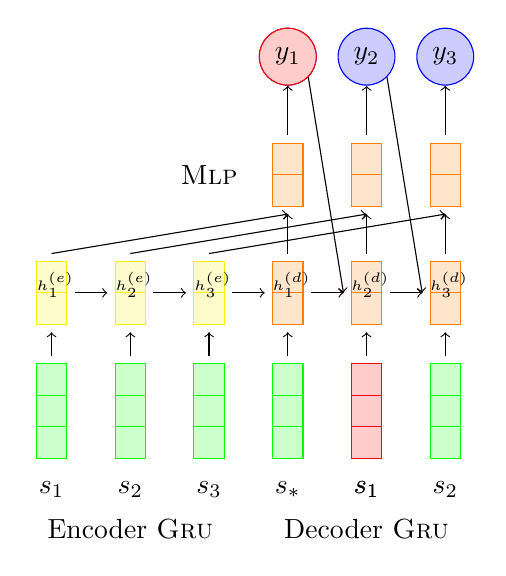
\begin{tikzpicture}[
  hid/.style 2 args={
    rectangle split,
    draw=#2,
    rectangle split parts=#1,
    fill=#2!20,
    outer sep=1mm},
  mlp/.style 2 args={
    rectangle split,
    rectangle split horizontal,
    draw=#2,
    rectangle split parts=#1,
    fill=#2!20,
    outer sep=1mm}
]

 \foreach \i [count=\step from 1] in {$s_1$, $s_2$, $s_3$, $s_*$, $s_1$, $s_2$}
    \node (i\step) at (1*\step, -2) {\i};
  % draw embedding and hidden layers for text input
  \foreach \step in {1,...,3} {
    \node[hid={3}{green}] (e\step) at (1*\step, -1) {};    
  }
    \node[hid={3}{green}] (e4) at (1*4, -1) {};    
  \foreach \step in {5,...,6} {
    \node[hid={3}{green}] (e\step) at (1*\step, -1) {};    
  }

  \foreach \step in {1,...,3} {
    \node[hid={2}{yellow}] (h_f_\step) at (1 *\step, .5) {};    
    \draw[->] (e\step.north) -> (h_f_\step.south);
  }

  \foreach \step in {1,...,3} {
      \node (hlbl\step) at (1*\step + .05, .6) {\tiny $h^{(e)}_\step$};    
  }


  \foreach \step in {4,...,6} {
    \node[hid={2}{orange}] (h_f_\step) at (1 *\step, .5) {};    
    \node[hid={2}{orange}] (g_f_\step) at (1 *\step, 2) {};    
    \draw[->] (e\step.north) -> (h_f_\step.south);
  }

  \foreach \step in {1,...,3} {
      \node (hlbl\step) at (1*\step + 3 + .05, .6) {\tiny $h^{(d)}_\step$};    
  }
  \foreach \step in {1,...,3} {
    \node[circle, draw=blue, fill=blue!20] (y_\step) at (3 + 1 *\step, 3.5) {$y_\step$};    
 }
    \draw[->] (y_1.south east) -> (h_f_5.west);
    \draw[->] (y_2.south east) -> (h_f_6.west);
    \draw[->] (h_f_4.north) -> (g_f_4.south);
    \draw[->] (g_f_4.north) -> (y_1.south);
    \draw[->] (h_f_5.north) -> (g_f_5.south);
    \draw[->] (g_f_5.north) -> (y_2.south);
    \draw[->] (h_f_6.north) -> (g_f_6.south);
    \draw[->] (g_f_6.north) -> (y_3.south);
 \foreach \step/\steppp in {1/2, 2/3, 3/4, 4/5, 5/6} {
   
    \draw[->] (h_f_\step.east) -> (h_f_\steppp.west);
  }
    \draw[->] (h_f_1.north) -> (g_f_4.south);
    \draw[->] (h_f_2.north) -> (g_f_5.south);
    \draw[->] (h_f_3.north) -> (g_f_6.south);

    \node (enc) at (2,-2.5) {Encoder \textsc{Gru}};
    \node (dec) at (5,-2.5) {Decoder \textsc{Gru}};
    \node (mlp) at (3, 2) {\textsc{Mlp}};

  \uncover<5->{
  \node (i5) at (1*5, -2) {\alert{$s_1$}};
    \node[circle, draw=red, fill=red!20] (y_1) at (3 + 1 *1, 3.5) {$y_1$};    
    \node[hid={3}{red}] (e5) at (1*5, -1) {};    
}

\end{tikzpicture}

%    \end{column}
%    \begin{column}{0.5\textwidth}
%      \begin{align*}
%        \uncover<1->{p(y|h) &= \prod_{i=1}^n p(y_i|y_{<i}, h^{(d)}_{<i}, 
%                                                       h^{(e)} )}\\
%        \uncover<2->{p_i & \triangleq p(y_i=1|h) = 
%                            \textsc{Mlp}([h^{(e)}_i; h^{(d)}_i])}\\
%        \uncover<3->{h^{(d)}_i &= \textsc{Gru}\left(h_{i-1}^{(d)},  
%                                 \alert<5->{p_{i-1} \cdot  s_{i-1}}\right)}
%      \end{align*}
%    \end{column}
%  \end{columns}
%\end{frame}
%
%\begin{frame}{Sentence Extractor}
%  \textbf{Previous Work}\\~\\
%  ~~ -- \textbf{Cheng and Lapata Extractor} ~~ seq2seq inspired architecture 
%                                               (Cheng and Lapata, 2016)\\
%  ~~ -- \alert{\textbf{SummaRunner Extractor}} ~~ RNN inspired architecture 
%                                                  with document and summary 
%                                                  representations 
%                                                  (Nallapati et al., 2016)\\
%  ~\\~\\
%  \textbf{Our Extractors}\\~\\
%  ~~ -- \textbf{RNN Extractor} ~~ Simplified version of SummaRunner \\
%  ~~ -- \textbf{Seq2Seq Extractor} ~~ seq2seq (with attention) inspired 
%                                      architecture \\
%\end{frame}
%
%
%
%\begin{frame}{SummaRunner Extractor}
%  \begin{columns}
%    \begin{column}{0.5\textwidth}
%      \documentclass[tikz,border=10pt]{standalone}
\usetikzlibrary{shapes}
\usetikzlibrary{arrows}
\usetikzlibrary{positioning}
\begin{document} 

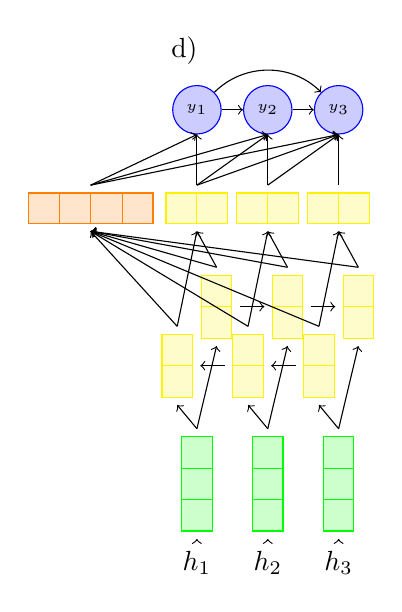
\begin{tikzpicture}[
  hid/.style 2 args={
    rectangle split,
    draw=#2,
    rectangle split parts=#1,
    fill=#2!20,
    outer sep=1mm},
  mlp/.style 2 args={
    rectangle split,
    rectangle split horizontal,
    draw=#2,
    rectangle split parts=#1,
    fill=#2!20,
    outer sep=1mm}
]

  \node [anchor=west] (label) at (.45, 4.5) {d)};
 \foreach \i [count=\step from 1] in {$h_1$, $h_2$, $h_3$}
    \node (i\step) at (.9*\step, -2) {\i};
  % draw embedding and hidden layers for text input
  \foreach \step in {1,...,3} {
    \node[hid={3}{green}] (e\step) at (.9*\step, -1) {};    
    \draw[->] (i\step.north) -> (e\step.south);
  }

        \node[mlp={4}{orange}] (h_0) at (.9 *-.5, 2.5) {};    
  \foreach \step in {1,...,3} {
    \node[hid={2}{yellow}] (h_f_\step) at (.25 + .9 *\step, 1.25) {};    
    \node[hid={2}{yellow}] (h_r_\step) at (-.25 + .9 *\step, .5) {};    
    \draw[->] (h_r_\step.north) -> (h_0.south);
    \draw[->] (h_f_\step.north) -> (h_0.south);
    \draw[->] (e\step.north) -> (h_f_\step.south);
    \draw[->] (e\step.north) -> (h_r_\step.south);
    \node[mlp={2}{yellow}] (h_\step) at (.9 *\step, 2.5) {};    
    \node[circle, draw=blue, fill=blue!20] (y_\step) at (.9 *\step, 3.75) {\tiny $y_\step$};    
    \draw[->] (h_\step.north) -> (y_\step.south);
    \draw[->] (h_f_\step.north) -> (h_\step.south);
    \draw[->] (h_r_\step.north) -> (h_\step.south);
  }

  \foreach \step/\steppp in {1/2, 2/3} {
    \draw[->] (h_f_\step.east) -> (h_f_\steppp.west);
    \draw[->] (h_r_\steppp.west) -> (h_r_\step.east);
  }
 
    \draw[->] (h_0.north) -> (y_1.south);
    \draw[->] (h_0.north) -> (y_2.south);
    \draw[->] (h_0.north) -> (y_3.south);
    \draw[->] (y_1.east) -> (y_2.west);
    \draw[->] (y_2.east) -> (y_3.west);
    \draw[->] (h_1.north) -> (y_2.south);
    \draw[->] (h_1.north) -> (y_3.south);
    \draw[->] (h_2.north) -> (y_3.south);
    \draw [bend left=45,->] (y_1) to (y_3);
\end{tikzpicture}


\end{document}

%    \end{column}
%    \begin{column}{0.5\textwidth}
%      $d = \tanh\big(b_d + W_d \frac{1}{n} \sum_{i=1}^n h_i   \big) $\\
%      $ g_i  = \sum_{j=1}^{i-1} p(y_j=1|y_{<j},h) \cdot h_j$\\
%      \begin{align*}
%        \textit{content}  \quad a^{(con)}_i & =W^{(con)} h_i \\
%        \textit{salience} \quad a^{(sal)}_i & = h_i^TW^{(sal)} d \\
%        \textit{novelty} \quad a^{(nov)}_i & = -h_i^TW^{(nov)} \tanh(g_i) 
%                    \label{eq:srnov} \\
%        \textit{position} \quad a^{(pos)}_i & = W^{(pos)} l_i \\
%        \textit{quartile} \quad a^{(qrt)}_i & = W^{(qrt)} r_i
%      \end{align*}
%      $p(y_i|y_{<i}, h) = \sigma\left(\begin{array}{l} a^{(con)}_i 
%        +a^{(sal)}_i + a^{(nov)}_i+ \\ a^{(pos)}_i + a^{(qrt)}_i + 
%         b \end{array}\right) $ \\
%    \end{column}
%  \end{columns}
%\end{frame}




\section{Data}

\begin{frame}{Datasets - News}
  \begin{center}
    \begin{tabular}{ rfrfr }
      \toprule
      \textbf{Dataset} & \textbf{Train} & \textbf{Valid} & \textbf{Test} &
        \textbf{Refs} \\
        \midrule
        CNN/DailyMail & 287,113 & 13,368 & 11,490 & 1\\
        NYT & 44,382 & 5,523 & 6,495 & 1.93\\
        DUC 2001/2002 & 516 & 91 & 657 & 2 \\
      \bottomrule
    \end{tabular}
  \end{center} 
  ~\\

  Sizes of the training, validation, test splits for each dataset
  and the average number of test set human reference summaries per document.

\end{frame}

\begin{frame}{Datasets - Non-News}
  \begin{center}
    \begin{tabular}{ rfrfrf }
      \toprule
      \textbf{Dataset} & \textbf{Genre} & 
        \textbf{Train} & \textbf{Valid} & \textbf{Test} &
        \textbf{Refs} \\
        \midrule
        Reddit & Personal Narratives & 404 & 24 & 48 & 2 \\
        AMI & Office Meetings & 98 & 19 & 20 & 1 \\
        PubMed & Medical Journal Articles& 21,250 & 1,250 & 2,500 & 1\\
      \bottomrule
    \end{tabular}
  \end{center} 
  ~\\

  Sizes of the training, validation, test splits for each dataset
  and the average number of test set human reference summaries per document.


\end{frame}


\section{Experiments}

\begin{frame}{Experiments}
%
    \alert<4>{\textbf{Main Experiment}}\\
    Evaluate encoder/extractor pairs using ROUGE-2 recall.\\
%
  \begin{columns}
    \begin{column}{0.3\textwidth}
    \uncover<5->{\textbf{Additional Experiments}}    
      \begin{itemize}
        \uncover<5->{\item \alert<5>{fine-tuned embeddings}}
        \uncover<6->{\item \alert<6>{word class ablations}}
        \uncover<7->{\item \alert<7>{sentence order shuffling}}
      \end{itemize}
    \end{column}
    \begin{column}{0.7\textwidth}
        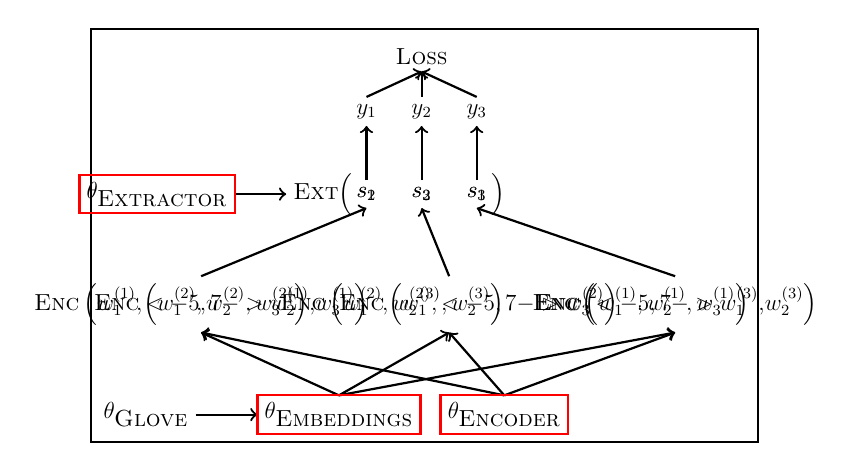
\begin{tikzpicture}[thick,scale=0.7, every node/.style={transform shape}]

  \draw[draw=black] (-2,5) rectangle (10.1,-2.5);

  \uncover<1-6>{
    \node (w1) at (0,0) 
      {\large $\textsc{Enc}\left(w^{(1)}_1,
       \uncover<-5,7->{w^{(1)}_2,} w^{(1)}_3\right)$};
    \node (w3) at (8.6,0) 
      {\large $\textsc{Enc}\left( \uncover<-5,7->{ w^{(3)}_1, }
       w^{(3)}_2 \right)$};
    \node (w2) at (4.5,0) 
      {\large $\textsc{Enc}\left(w^{(2)}_1, 
       w^{(2)}_2,\uncover<-5,7->{  w^{(2)}_3} \right)$};


  }
  
  \uncover<7>{
    \node (w21) at (0,0) 
      {\large $\textsc{Enc}\left(w^{(2)}_1, w^{(2)}_2,w^{(2)}_3 \right)$};
    \node (w13) at (8,0) 
      {\large $\textsc{Enc}\left(w^{(1)}_1, w^{(1)}_2, w^{(1)}_3\right)$};
    \node (w32) at (4,0) 
      {\large $\textsc{Enc}\left(w^{(3)}_1, w^{(3)}_2 \right)$};
  }





  \uncover<1-6>{
    \node (s1) at (3,2) {\large $s_1$};
    \node (s2) at (4,2) {\large $s_2$};
    \node (s3) at (5,2) {\large $s_3$};
  }
  \uncover<7>{
    \node (s13) at (5,2) {\large $s_1$};
    \node (s21) at (3,2) {\large $s_2$};
    \node (s32) at (4,2) {\large $s_3$};
  }


    \draw[->,thick] (w1.north) -- (s1.south); 
    \draw[->,thick] (w2.north) -- (s2.south);
    \draw[->,thick] (w3.north) -- (s3.south);

    \node (ext) at (3.6,2) {\large $\textsc{Ext}\Big( 
        \quad\quad\quad\;\;\;\;\;\;\;\;\;\;\; \Big)$};
\uncover<2->{
    \node (extp) at (-.8,2) {\large $\theta_\textsc{Extractor}$};
    \node (encp) at (5.5,-2) {\large $\theta_\textsc{Encoder}$};
    \draw[->,thick] (encp.north) -- (w1.south);
    \draw[->,thick] (encp.north) -- (w2.south);
    \draw[->,thick] (encp.north) -- (w3.south);
    \draw[->,thick] (extp.east) -- (ext.west);
}

\uncover<3->{
    \node (embp) at (2.5,-2) {\large $\theta_\textsc{Embeddings}$};
    \draw[->,thick] (embp.north) -- (w1.south);
    \draw[->,thick] (embp.north) -- (w2.south);
    \draw[->,thick] (embp.north) -- (w3.south);
}
\uncover<4->{
        \draw[draw=red] (extp.north east) rectangle (extp.south west);
       \draw[draw=red] (encp.north east) rectangle (encp.south west);
    \node (glovep) at (-1,-2) {\large $\theta_\textsc{Glove}$};
    \draw[->,thick] (glovep.east) -- (embp.west);

}
\uncover<5>{
        \draw[draw=red] (embp.north east) rectangle (embp.south west);
}
    \node (y1) at (3,3.5) {\large $y_1$};
    \node (y2) at (4,3.5) {\large $y_2$};
    \node (y3) at (5,3.5) {\large $y_3$};
    \draw[->,thick] (s1.north) -- (y1.south);
    \draw[->,thick] (s2.north) -- (y2.south);
    \draw[->,thick] (s3.north) -- (y3.south);

    \node (loss) at (4, 4.5) {\large \textsc{Loss}};
    \draw[->,thick] (y1.north) -- (loss.south);
    \draw[->,thick] (y2.north) -- (loss.south);
    \draw[->,thick] (y3.north) -- (loss.south);
 

%    \uncover<2->{   
 %      \draw[->,thick,red] (loss.south) + (-5mm, 0) -- (y1.north west);
 %      \draw[->,thick,red] (loss.south) + (5mm, 0) -- (y3.north east);
 %   }
 %   \uncover<3->{
 %      \draw[->,thick,red] (y1.north west) -- (s1.north west);
 %      \draw[->,thick,red] (y3.north east) -- (s3.north east);
 %   }
 %   \uncover<4->{
 %      \draw[->,thick,red] (s1.north west) -- (extp.north east) ;
 %   }
 %   \uncover<5->{
 %      \draw[->,thick,red] (s1.south west)+(-5mm,0) -- (-.7, .6) ;
 %      \draw[->,thick,red] (s3.south east)+(5mm,0) -- (9.2, .6) ;
 %   }
%    \uncover<6->{
 %      \draw[->,thick,red] (-.7, -.5) -- (encp.north west) ;
 %      \draw[->,thick,red] (9.2, -.5) -- (encp.north east) ;
 %      \draw[->,thick,red] (w2.south)+(-2mm,0) -- (4.3, -1.5) ;
  %  }
    

\end{tikzpicture}
 
    \end{column}
  \end{columns}
\end{frame}

\begin{frame}{Model Training}

    Maximum Likelihood training using gold extract summaries.

    \[\max_{\theta} \frac{1}{|\mathcal{D}|} \sum_{(s,y^*)\in \mathcal{D}} 
    \log p(y^*| s) \]

   
    ~\\

    Gold extract summaries $y^*$ heuristically created by maximizing ROUGE-1 recall.

\end{frame}

\begin{frame}{Summary Generation}

    \begin{enumerate}
        \item Rank sentences $s_i$ in decreasing order by $p(y_i=1|h)$.
        \item Create a summary by extracting the top ranked sentences until a word length budget.
    \end{enumerate}

\end{frame}


\section{Results}


\begin{frame}{Choice of Sentence \alert{Enc}oder: News}
  \begin{center}
      \begin{tabular}{ccgcg} 
        & & \multicolumn{3}{c}{\textbf{Rouge-2 Recall}}\\
      \toprule
      \textbf{\textsc{Ext}} & \alert{\underline{\textbf{\textsc{Enc}}}}
          & \textbf{CNN/DM} & \textbf{NYT} & \textbf{DUC} \\
      \midrule
      \textsc{Lead}   
         & --         &        $24.4$ &        $32.3$ &   $21.5$  \\
      \hline 
      \multirow{3}{*}{\textsc{Seq2Seq}}
         &\textsc{Avg}&
           \alert{\textbf{25.6}}&\textbf{35.7}&\alert{\textbf{22.8}}  \\
         &\textsc{Rnn}&        25.3 &\textbf{35.9}&        22.5   \\
         &\textsc{Cnn}&        25.1 &        35.1 &\textbf{22.7}  \\
         \hline
      \multirow{3}{*}{\textsc{Cheng \& Lapata}}
         &\textsc{Avg}&
           \alert{25.3}&\textbf{35.6}&\alert{\textbf{23.1}}\\
         &\textsc{Rnn}&        
                     25.0 &          \textbf{35.8} &          \textbf{23.0} \\
         &\textsc{Cnn}&       
                     25.1 &                  35.0  &          \textbf{23.0} \\
         \hline
      \textsc{Oracle} 
         & --         &          36.2 &        48.9 &        31.8   \\
      \bottomrule
    \end{tabular}
    
  \end{center}
  ~\\

  Averaging is either the \alert{\textbf{best}} encoder or 
  \textbf{statistically indistinguishable} from the best encoder!

\end{frame}

\begin{frame}{Choice of Sentence \alert{Enc}oder: Non-News}
  \begin{center}
    \begin{tabular}{ccgcg} 
        & & \multicolumn{3}{c}{\textbf{Rouge-2 Recall}}\\
  \toprule
  \textbf{\textsc{Ext}} & \textbf{\textsc{Enc}} 
      & \textbf{Reddit} & \textbf{AMI} & \textbf{PubMed} \\
  \midrule
  \textsc{Lead}   
     & --         &        $\mathbf{10.9}$ &        $2.0$ &   $9.3$  \\
  \hline
  \multirow{3}{*}{\textsc{Seq2Seq}}
     &\textsc{Avg}&
                   \alert{\textbf{13.6}}&\alert{\textbf{5.5}}&\alert{\textbf{17.7}} \\
     &\textsc{Rnn}&
                   \textbf{12.0}&\textbf{5.3}&        16.7  \\
     &\textsc{Cnn}&
                   \textbf{13.2}&        2.9&        16.9  \\
     \hline
  \multirow{3}{*}{\textsc{Cheng \& Lapata}}
     &\textsc{Avg}&
       \alert{\textbf{13.6}} & \alert{\textbf{6.1}}   & \alert{\textbf{17.7}}\\
     &\textsc{Rnn}&       
       \textbf{12.6} & \textbf{5.0}   & 16.7\\
     &\textsc{Cnn}&       
       \textbf{13.4} & 2.8               &  16.9      \\
     \hline
  \textsc{Oracle} 
     & --         &       16.2    &    3.9     &       25.0   \\
  \bottomrule
\end{tabular}

    
  \end{center}
  ~\\

  Averaging is either the \alert{\textbf{best}} encoder or 
  \textbf{statistically indistinguishable} from the best encoder!
\end{frame}

\begin{frame}{Choice of Sentence \alert{Ext}ractor: News}
    
 \begin{center}
   \begin{tabular}{ccgcg}
 & & \multicolumn{3}{c}{\textbf{Rouge-2 Recall}}\\
 \toprule
 \textbf{Ext} & \textbf{Enc} & 
   \textbf{CNN/DM} & \textbf{NYT} & \textbf{DUC} \\
 \midrule
 \textsc{Lead}    &  --          & 
                   24.4  & 32.3  & 21.5 \\
 \hline
 \textsc{RNN}     & \textsc{Avg} &  
                   25.4  & 34.7  & 22.7 \\
 \hline
 \textsc{Seq2Seq} & \textsc{Avg} & 
           \alert{\textbf{25.6}} & \alert{\textbf{35.7}} & \textbf{22.8} \\
 \hline
 \textsc{Cheng \&  Lapata} & \textsc{Avg} & 
                    25.3 & \textbf{35.6} & \textbf{23.1} \\
 \hline
 \textsc{SummaRunner}  & \textsc{Avg} &  
                    25.4 & 35.4 & 22.3 \\
 \hline
    \textsc{Oracle} & -- & 36.2 &  48.9 &  31.8\\
 \bottomrule
\end{tabular}

 \end{center}
 
 ~\\

 \textsc{Seq2Seq} is the \alert{\textbf{best}} or \textbf{statistically 
 indistinguishable} from the best system.

 ~\\
 \textsc{Rnn} extractor as good as \textsc{SummaRunner} or 
 \textsc{Cheng \& Lapata} extractors on CNN/DailyMail data.

  

\end{frame}

\begin{frame}{Choice of Sentence \alert{Ext}ractor: Non-News}
    
 \begin{center}
   \begin{tabular}{ccgcg}
 & & \multicolumn{3}{c}{\textbf{Rouge-2 Recall}}\\
\toprule
\alert{\underline{\textbf{Ext}}} & \textbf{Enc} & 
   \textbf{Reddit} & \textbf{AMI} & \textbf{PubMed} \\
\midrule
\textsc{Lead}    &  --          & 
                   \textbf{10.9}  & 2.0  & 9.3 \\
\hline
\textsc{Rnn}     & \textsc{Avg} &  
                   \textbf{11.4}  & \textbf{5.5}  & 17.0 \\
\hline
\textsc{Seq2Seq} & \textsc{Avg} & 
           \alert{\textbf{13.6}} & \textbf{5.5} & \textbf{17.7} \\
\hline
\textsc{Cheng \&  Lapata} & \textsc{Avg} & 
           \textbf{13.6} & \textbf{6.1} & \textbf{17.7} \\
\hline
\textsc{SummaRunner}  & \textsc{Avg} &  
           \textbf{13.4} & \textbf{5.6} & \textbf{17.2} \\
\hline
    \textsc{Oracle} & -- & 16.2 &  3.9 &  25.0\\
\bottomrule
\end{tabular}


 \end{center}

 ~\\

 \textsc{Seq2Seq} is the \alert{\textbf{best}} or statistically indistinguishable from the best
 system.


\end{frame}



\begin{frame}{Word Embedding Fine-Tuning: (News)}
  \begin{center}
    \begin{tabular}{ccccc}
      & & \multicolumn{3}{c}{\textbf{Rouge-2 Recall}}\\
      \toprule
        \textbf{Ext} & \textbf{Emb}  & 
           \textbf{CNN/DM} & 
           \textbf{NYT} & 
           \textbf{DUC} \\
      \midrule
      \multirow{2}{*}{\textsc{Seq2Seq}} 
        & Fixed & \textbf{25.6} & \textbf{35.7} & \textbf{22.8} \\
        & Fine-Tuned &         25.3  & \textbf{35.7} & \textbf{22.9} \\
      \hline
      \multirow{2}{*}{\textsc{Cheng \& Lapata}} 
        & Fixed & \textbf{25.3} & \textbf{35.6} & \textbf{23.1} \\
        & Fine-Tuned &         24.9  &         35.4  & \textbf{23.0} \\
      \bottomrule
  \end{tabular}


 \end{center}

 ~\\
 
% Performance difference when using \textit{fixed} embeddings versus 
% \textit{fine-tuned} embeddings.
 
  ~\\

%  Models are using the \textsc{Avg} encoder and are initialized with 
%  Glove embeddings. 

%  ~\\

  \textbf{No statistically significant improvement} on news with fine-tuning!

\end{frame}

\begin{frame}{Word Embedding Fine-Tuning: Non-News}
 \begin{center}
  \begin{tabular}{ccccc}
   & & \multicolumn{3}{c}{\textbf{Rouge-2 Recall}}\\
   \toprule
   \textbf{Ext} & \textbf{Emb}  & 
        \textbf{Reddit} & \textbf{AMI} & \textbf{PubMed} \\
   \midrule
   \multirow{2}{*}{\textsc{Seq2Seq}}
      & Fixed & \textbf{13.6} &         5.5  & \textbf{17.7} \\
      & Fine-Tuned & \textbf{13.8} & \textbf{5.8} &         16.9  \\
   \hline
   \multirow{2}{*}{\textsc{Cheng \& Lapata}} 
      & Fixed & \textbf{13.6} & \textbf{6.1} & \textbf{17.7} \\
      & Fine-Tuned & \textbf{13.4} & \textbf{6.2} & \textbf{16.4} \\
   \bottomrule
  \end{tabular}


 \end{center}

 ~\\
 
% Performance difference when using \textit{fixed} embeddings versus 
% \textit{fine-tuned} embeddings.
 
 ~\\

% All models are using the \textsc{Avg} encoder and are initialized with 
% pretrained Glove embeddings from gigaword/wikipedia. 

% ~\\
 \textbf{Statistically significant improvement} with \textsc{Seq2Seq} on AMI
 data. (Caveat: only speech dataset)\\

~\\
Otherwise, same trend as news, \textbf{no stat. sig. improvement} using fine-tuning.

\end{frame}

\begin{frame}{Word Class Ablation: ROUGE-2 Recall}
 \begin{center}
  \begin{tabular}{lcccccc}
   \toprule
   \multirow{1}{*}{\textbf{Ablation}} & 
            \textbf{CNN/DM} & \textbf{NYT} & \textbf{DUC} &
            \textbf{Reddit} & \textbf{AMI} & \textbf{PubMed} \\
   \midrule
     All Words & $\mathbf{25.4}$ & $\mathbf{34.7}$ & $22.7$ &
                  $\mathbf{11.4}$ & $5.5$ & $\mathbf{17.0}$  \\
   \uncover<2->{$-$ Nouns & $25.3$  & $34.3 $ & $22.3$  &
   \alert<2>{$10.3$} & \alert<2>{$3.8$} & \alert<2>{$15.7$}} \\
   \uncover<2->{$-$ Verbs & $25.3$  & $34.4 $ & $22.4$ &
            $10.8$ & $5.8$ & $16.6$ }\\
   \uncover<3->{$-$ Adj/Adv & 
  $25.3$ & $34.4$ & $22.5$ &
   \alert<3>{$9.5$} & $5.4$ & $16.8$} \\
   \uncover<4->{$-$ Function & $25.2$ & $34.6$ & \alert<4>{$\mathbf{22.9}$} &
   $10.3$ & \alert<4>{$\mathbf{6.3}$} & $16.6$ }\\
   \bottomrule
  \end{tabular}
 \end{center}


 %RNN extractor with Averaging encoder. 

 %~\\


 \uncover<2->{\textbf{-Nouns/Verbs} Doesn't decrease performance much on News. Non-News sees small performance drops. }

~\\ 

 \uncover<3->{\textbf{-Adj/Adv} Intensifiers are important in personal stories.
 Signal climactic and important moments.}


 ~\\

 \uncover<4->{\textbf{-Function} Possibly noisy signals on small datasets.}



 ~\\
 \uncover<1-5>{\tiny{\textbf{Bold} is best performance.}}

\end{frame}



\begin{frame}{Shuffled vs In-Order (News)}

 \begin{center}
  \begin{tabular}{ccL{2cm}m{1cm}L{.75cm}} 
   \toprule
   \textbf{Ext.} & \textbf{Order} & 
                           \textbf{CNN/DM} & \textbf{NYT} & \textbf{DUC} \\
   \midrule
%?   \multirow{2}{*}{RNN} 
%?       & In-Order & 
%?       \textbf{25.4} & \textbf{34.7} & \textbf{22.7} \\
%?       & Shuffled & 
%?               22.8 &          25.0  &         18.2  \\
   \multirow{2}{*}{Seq2Seq}
       & In-Order & 
       \textbf{25.6} & \textbf{35.7} &  \textbf{22.8} \\
       & Shuffled & 
               21.7  &         25.6  &          21.2  \\
   \bottomrule
  \end{tabular}
 \end{center}

 ~\\

 Shuffled model is trained on shuffled sentence order documents.

 ~\\

 Both models evaluated on in-order data.


~\\ 
 Large \textbf{performance drops} on news!

\end{frame}

\begin{frame}{Shuffled vs In-Order (Other)}

 \begin{center}
  \begin{tabular}{ccccc} 
   \toprule
   \textbf{Ext.} & \textbf{Order} & 
                           \textbf{Reddit} & \textbf{AMI} & \textbf{PubMed} \\
   \midrule
   \multirow{2}{*}{Seq2Seq}
       & In-Order & 
       \textbf{13.6} &         5.5  &  \textbf{17.7} \\
       & Shuffled & 
       \textbf{13.5} & \textbf{6.0} &          14.9  \\
   \bottomrule
  \end{tabular}
 \end{center}

 ~\\

 Shuffled model is trained on shuffled sentence order documents.

 ~\\

 Both models evaluated on in-order data.

 ~\\

 Small \textbf{performance increase} on AMI.

\end{frame}



\begin{frame}

    Summary of Findings:
    \begin{itemize}
        \item<1-> Sentence position dominates the learning signal. 
        \item<2-> Word/Sentence embeddings contain shallow semantics; need better representation for summarization task.
        \item<4-> Richer features are better than richer models.
        \item<5-> Simpler is good enough:
            \begin{itemize}
        \item<6-> Averaging sentence encoder is as good as RNNs or CNNs.
        \item<7-> RNN extractor on par with more complicated models.
    \end{itemize}
    \end{itemize}

    \uncover<8->{

~\\

~\\

        \textbf{Thank you for listening! Ask me questions!}


        ~\\
        Code and data at: \url{https://github.com/kedz/nnsum/tree/emnlp18-release} \\
        or \url{http://cs.columbia.edu/\~kedzie}

    }


\end{frame}



\end{document} 
